\chapter{METHODOLOGIES ET MODELES}
\thispagestyle{empty}
\label{chap:methodologies-modeles-fr}

% Pour les diagrammes de flux de ce chapitre, il faut ajouter
% \usepackage{tikz} dans le preambule du fichier .tex principal.

\nomenclature{API}{Application Programming Interface}
\nomenclature{BLEU}{Bilingual Evaluation Understudy}
\nomenclature{METEOR}{Metric for Evaluation of Translation with Explicit ORdering}
\nomenclature{mBART}{Multilingual Bidirectional and Auto-Regressive Transformer}
\nomenclature{mT5}{Massively Multilingual Text-to-Text Transfer Transformer}
\nomenclature{ROUGE}{Recall-Oriented Understudy for Gisting Evaluation}
\nomenclature{RSS}{Really Simple Syndication}
\nomenclature{XL-Sum}{Large-scale Multilingual Abstractive Summarization}

\section{Approche methodologique generale}

La conception methodologique de ce projet repose sur trois couches principales: la preparation et l'entrainement des modeles, l'evaluation des modeles avec des metriques multidimensionnelles, et l'integration des modeles selectionnes dans une application web fournissant un flux d'actualites en temps reel. Cette structure permet au projet de ne pas rester seulement une etude d'entrainement de modele, mais de devenir un systeme de bout en bout fonctionnant avec de vraies sources d'actualites.

Dans la premiere couche, des modeles transformeurs de type sequence-a-sequence adaptes au resume d'actualites ont ete etudies, et des modeles multilingues bases sur mBART ont ete entraines dans le cadre du projet. Des modeles bases sur BART ont aussi ete prepares pour des experiences de resume en anglais, mais l'objectif principal du scenario multilingue reste les modeles mBART. Le modele base sur mT5 n'a pas ete reentraine dans ce projet; il a ete pris comme modele pret a l'emploi, deja entraine dans une etude similaire, et utilise pour la comparaison.

Dans la deuxieme couche, les modeles ont ete evalues non seulement avec des metriques classiques de similarite textuelle, mais aussi avec des signaux supplementaires comme la fidelite a la source, le comportement de repetition, la lisibilite, la couverture de l'information, la compression et le temps d'execution. Pour cette raison, en plus des metriques classiques comme ROUGE, BLEU et METEOR-lite, des scores proxy composites ont ete definis dans le cadre du projet. Dans la troisieme couche, les modeles ont ete integres dans une application qui collecte des nouvelles depuis des sources RSS, extrait le corps des articles, pre-calcule les resumes, les stocke dans une base SQLite et les presente a l'utilisateur via une interface web.

Figure~\ref{fig:methodology-overview-fr} presente le flux methodologique general du projet.

\begin{figure}[t]
\centering
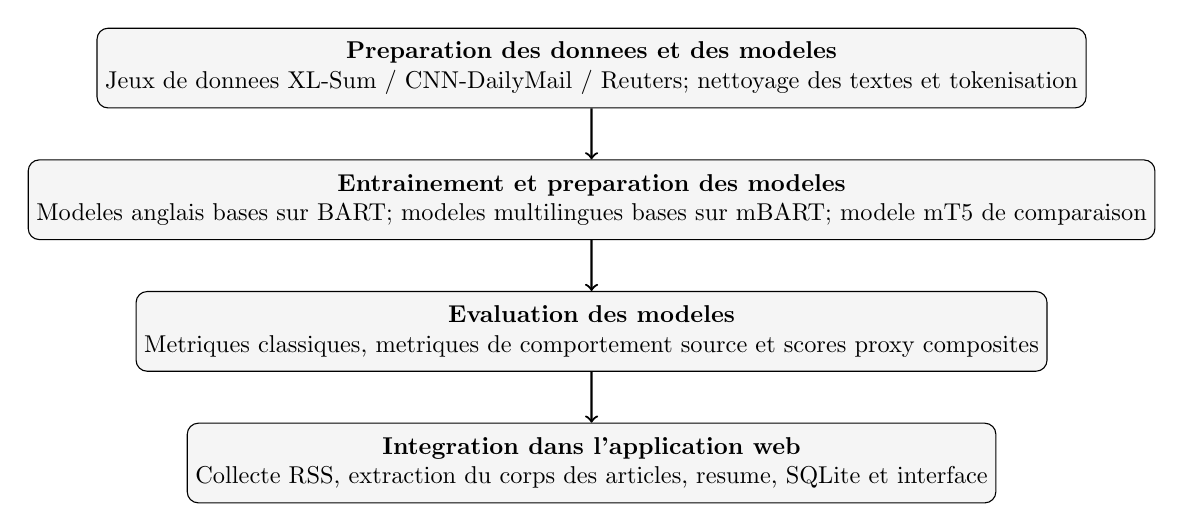
\begin{tikzpicture}[
  scale=0.88,
  every node/.style={transform shape},
  box/.style={draw, rounded corners, align=center, minimum width=10.8cm, minimum height=1.15cm, fill=gray!8},
  arrow/.style={->, thick}
]
\node[box] (data) at (0,0) {
  \textbf{Preparation des donnees et des modeles}\\
  Jeux de donnees XL-Sum / CNN-DailyMail / Reuters; nettoyage des textes et tokenisation
};
\node[box] (train) at (0,-1.9) {
  \textbf{Entrainement et preparation des modeles}\\
  Modeles anglais bases sur BART; modeles multilingues bases sur mBART; modele mT5 de comparaison
};
\node[box] (eval) at (0,-3.8) {
  \textbf{Evaluation des modeles}\\
  Metriques classiques, metriques de comportement source et scores proxy composites
};
\node[box] (app) at (0,-5.7) {
  \textbf{Integration dans l'application web}\\
  Collecte RSS, extraction du corps des articles, resume, SQLite et interface
};
\draw[arrow] (data) -- (train);
\draw[arrow] (train) -- (eval);
\draw[arrow] (eval) -- (app);
\end{tikzpicture}
\caption{Flux methodologique general du projet}
\label{fig:methodology-overview-fr}
\end{figure}

\section{Sources de donnees et couverture linguistique}

Des sources de donnees orientees vers le resume d'actualites ont ete utilisees pour l'entrainement et l'evaluation des modeles. La famille XL-Sum constitue la source principale pour le resume multilingue. Dans la premiere chaine d'entrainement mBART, le jeu de donnees \texttt{GEM/xlsum} a ete utilise. Dans la deuxieme chaine d'entrainement mBART, le jeu de donnees \texttt{csebuetnlp/xlsum} a ete prefere. Ce choix a permis de construire une deuxieme chaine plus proche de l'organisation de XL-Sum et de ses longueurs cibles de resume.

Le plan d'evaluation du projet contient 15 langues: anglais, turc, francais, allemand, espagnol, italien, russe, arabe, hindi, chinois, japonais, coreen, neerlandais, roumain et vietnamien. Cependant, dans la version publique utilisee de \texttt{csebuetnlp/xlsum}, les sous-ensembles correspondant a l'allemand, l'italien, le neerlandais et le roumain n'etaient pas disponibles; ces langues ont donc ete ignorees dans l'execution d'evaluation. L'evaluation complete finale a ete realisee sur 11 langues et 52.219 exemples de test.

Dans la couche applicative, la source de donnees n'est pas un jeu de donnees academique fixe, mais des sources d'actualites RSS. Le systeme collecte les entrees RSS definies pour chaque langue, ouvre le lien de l'article, tente d'extraire le corps complet de l'article et envoie le texte nettoye au modele de resume. Ainsi, un lien est etabli entre les jeux de donnees reguliers utilises pour l'entrainement et l'evaluation, et les flux d'actualites reels utilises dans l'application.

\section{Familles de modeles et choix des modeles}

Les modeles utilises dans le projet sont regroupes en trois categories. La premiere categorie contient les modeles bases sur BART pour le resume d'actualites en anglais. Elle comprend les modeles \texttt{bart\_large\_cnn}, \texttt{bart\_base\_cnn} et \texttt{bart\_reuters}. La deuxieme categorie contient les modeles multilingues bases sur mBART entraines dans le cadre du projet: \texttt{mbart50\_xlsum} et \texttt{mbart-xlsum-2}. La troisieme categorie correspond au modele mT5 pret a l'emploi utilise pour la comparaison: \texttt{mt5-xlsum}.

Tableau~\ref{tab:model-families-fr} resume les groupes de modeles utilises dans le projet.

\begin{table}[t]
\caption{Familles de modeles utilisees dans le projet}
\label{tab:model-families-fr}
\centering
\begin{tabular}{|p{3.2cm}|p{4.1cm}|p{6.2cm}|}
\hline
\textbf{Groupe de modeles} & \textbf{Cles de modele} & \textbf{Role dans le projet} \\
\hline
Modeles bases sur BART & \texttt{bart\_large\_cnn}, \texttt{bart\_base\_cnn}, \texttt{bart\_reuters} & Modeles prepares pour le resume d'actualites en anglais. Ils sont utilises pour des experiences et comparaisons en anglais, pas comme solution principale multilingue. \\
\hline
Modeles bases sur mBART & \texttt{mbart50\_xlsum}, \texttt{mbart-xlsum-2} & Modeles multilingues entraines dans le cadre du projet. Ils constituent la sortie principale du developpement de modeles. \\
\hline
Modele base sur mT5 & \texttt{mt5-xlsum} & Modele non entraine dans ce projet. Il est utilise comme modele de comparaison pret a l'emploi, entraine dans une etude similaire. \\
\hline
\end{tabular}
\end{table}

Dans l'application, seules les modeles multilingues sont autorises pour les langues autres que l'anglais. Cela evite d'appeler par erreur des modeles BART entraines pour l'anglais sur des textes turcs, arabes, chinois ou dans d'autres langues. Le modele par defaut de l'application est \texttt{mbart50\_xlsum}; le jeu de modeles par defaut pour la generation en arriere-plan contient \texttt{mbart50\_xlsum}, \texttt{mbart-xlsum-2} et \texttt{mt5-xlsum}.

\section{Entrainement des modeles}

\subsection{Premiere chaine d'entrainement mBART}

Dans la premiere chaine d'entrainement mBART, le modele de base \texttt{facebook/mbart-large-50-many-to-many-mmt} a ete utilise. Le jeu de donnees \texttt{GEM/xlsum} a ete choisi comme source de donnees. Les exemples de differentes langues ont ete combines et un code de langue mBART a ete ajoute a chaque exemple. La longueur maximale des textes sources a ete fixee a 512 tokens, et la longueur maximale des resumes cibles a 96 tokens.

Cette chaine d'entrainement a ete concue comme un premier entrainement sur Colab, prudent et executable. L'entrainement a ete realise sur 2 epochs avec un taux d'apprentissage de $3 \times 10^{-5}$. L'evaluation basee sur la generation a ete desactivee pendant l'entrainement, et le choix du meilleur checkpoint n'a pas ete applique. Cette decision a ete prise pour reduire le cout de calcul et obtenir une premiere sortie de modele multilingue.

\subsection{Deuxieme chaine d'entrainement mBART}

La deuxieme chaine d'entrainement mBART a ete concue avec une priorite plus forte sur la qualite. Elle utilise encore le modele de base \texttt{facebook/mbart-large-50-many-to-many-mmt}, mais le jeu de donnees est remplace par \texttt{csebuetnlp/xlsum}. La longueur cible des resumes a ete reduite a 64 tokens afin d'adopter un objectif de generation plus proche de XL-Sum.

Dans cette deuxieme chaine, l'entrainement a ete organise par nombre d'etapes plutot que par nombre d'epochs. Le nombre total d'etapes a ete fixe a 35.000, le taux d'apprentissage a $1 \times 10^{-4}$ et le nombre d'etapes de warmup a 5.000. L'optimizer \texttt{adafactor} et le scheduler \texttt{inverse\_sqrt} ont ete utilises. Le modele a ete evalue et sauvegarde toutes les 5.000 etapes. L'evaluation basee sur la generation a ete activee et le meilleur modele a ete choisi selon la valeur ROUGE-L.

Dans cette chaine, un reechantillonnage par langue a aussi ete applique pour rendre les langues a faibles ressources plus visibles pendant l'entrainement. La probabilite d'entrainement de chaque langue est definie comme proportionnelle au nombre d'exemples de cette langue eleve a la puissance $\alpha$:

\begin{equation}
p_l = \frac{n_l^{\alpha}}{\sum_{j \in L} n_j^{\alpha}}
\label{eq:language-smoothing-fr}
\end{equation}

Ici, $L$ represente l'ensemble des langues, $n_l$ le nombre d'exemples d'entrainement dans la langue $l$, et $p_l$ la probabilite de reechantillonnage de cette langue. Dans le projet, $\alpha=0.5$ a ete choisi. Cette valeur reduit la domination des langues a fortes ressources tout en augmentant la representation des langues a faibles ressources.

Tableau~\ref{tab:training-configs-fr} presente les principales differences entre les deux chaines d'entrainement mBART.

\begin{table}[t]
\caption{Principales differences entre les chaines d'entrainement mBART}
\label{tab:training-configs-fr}
\centering
\begin{tabular}{|p{4.0cm}|p{4.6cm}|p{4.6cm}|}
\hline
\textbf{Caracteristique} & \textbf{\texttt{mbart50\_xlsum}} & \textbf{\texttt{mbart-xlsum-2}} \\
\hline
Modele de base & \texttt{facebook/mbart-large-50-many-to-many-mmt} & \texttt{facebook/mbart-large-50-many-to-many-mmt} \\
\hline
Jeu de donnees & \texttt{GEM/xlsum} & \texttt{csebuetnlp/xlsum} \\
\hline
Longueur source & 512 tokens & 512 tokens \\
\hline
Longueur cible & 96 tokens & 64 tokens \\
\hline
Duree d'entrainement & 2 epochs & 35.000 etapes \\
\hline
Taux d'apprentissage & $3 \times 10^{-5}$ & $1 \times 10^{-4}$ \\
\hline
Optimizer / scheduler & Parametres Trainer par defaut & \texttt{adafactor} + \texttt{inverse\_sqrt} \\
\hline
Validation & Evaluation generate desactivee & Evaluation generate toutes les 5.000 etapes \\
\hline
Choix du checkpoint & Pas de selection du meilleur modele & Meilleur checkpoint selon ROUGE-L \\
\hline
Equilibrage linguistique & Melange standard & Smoothing linguistique avec $\alpha=0.5$ \\
\hline
\end{tabular}
\end{table}

\section{Methode de generation des resumes}

Dans l'application, la generation des resumes est realisee avec des parametres de generation qui dependent de la famille du modele et de la langue. Les textes sources sont d'abord nettoyes et limites a une fenetre d'entree de 3.500 caracteres. Lors de la tokenisation, les entrees sont limitees a 1.024 tokens. Pour les modeles mBART, le code de langue source approprie est configure et \texttt{forced\_bos\_token\_id} est utilise pour orienter la generation vers la langue cible.

Les parametres generaux de generation comprennent la longueur maximale du resume, la longueur minimale, le nombre de beams, la penalite de longueur, l'interdiction de repetitions et l'arret anticipe. Pour les modeles mBART, le reglage par defaut est une longueur maximale de 90 tokens, une longueur minimale de 24 tokens et 5 beams. Pour le turc, des reglages specifiques ont ete appliques afin de produire des resumes plus equilibres et plus complets: longueur maximale de 84 tokens, longueur minimale de 26 tokens, 6 beams, interdiction de repetition de 4-grammes et penalite de repetition plus elevee. Pour le modele mT5, la longueur maximale est de 84 tokens, la longueur minimale de 20 tokens, avec 4 beams et une interdiction de repetition de 2-grammes.

Les resumes produits sont ensuite post-traites. Dans cette etape, la repetition du titre au debut du resume est evitee, les resumes trop proches du titre sont rejetes, les sorties incompletes ou degradees sont nettoyees, et un resume extractif de secours est utilise en cas de sortie degeneree. Ainsi, lorsque le modele echoue, le systeme ne renvoie pas une reponse vide; il extrait plutot un court resume controle a partir du texte source.

\section{Methode d'evaluation}

\subsection{Jeu de donnees d'evaluation et plan des modeles}

Dans la chaine d'evaluation, la partie test du jeu de donnees \texttt{csebuetnlp/xlsum} a ete utilisee. Meme si le plan du projet contient 15 langues, les langues sans sous-ensemble disponible dans la version publique de XL-Sum ont ete exclues de l'evaluation. Ainsi, l'evaluation complete contient 11 langues et 52.219 exemples de test.

Les modeles evalues sont \texttt{mbart50\_xlsum}, \texttt{mbart-xlsum-2} et \texttt{mt5-xlsum}. Les modeles BART specifiques a l'anglais sont definis dans la chaine d'evaluation, mais le rapport se concentre principalement sur la comparaison des modeles multilingues. Le titre n'a pas ete ajoute a l'entree du modele pendant l'evaluation; le modele a produit les resumes uniquement a partir du corps de l'article. Cette decision est coherente avec le comportement de l'application, ou le titre est affiche separement dans l'interface et le modele recoit le corps de l'article comme entree de resume.

\subsection{Metriques classiques et comportementales}

Les metriques d'evaluation sont organisees en trois groupes. Le premier groupe contient les metriques classiques de recouvrement avec la reference: ROUGE-1, ROUGE-2, ROUGE-L, BLEU et METEOR-lite. Ces metriques mesurent la similarite entre le resume produit par le modele et le resume humain de reference.

Le deuxieme groupe contient les metriques de comportement liees a la source et a la generation. Il comprend \texttt{source\_coverage}, \texttt{source\_recall}, \texttt{fragment\_coverage}, \texttt{fragment\_density}, \texttt{novelty\_1gram}, \texttt{novelty\_2gram}, \texttt{repetition\_3gram}, \texttt{compression\_ratio}, \texttt{latency\_seconds} et \texttt{latency\_per\_1k\_tokens}. Ces metriques permettent d'analyser non seulement la similarite avec la reference, mais aussi la fidelite a la source, la tendance a la repetition, le degre d'abstraction, le comportement de compression et le temps d'execution.

\subsection{Scores proxy composites}

Le troisieme groupe correspond aux scores proxy composites concus dans le cadre du projet. Ces scores ne remplacent pas l'evaluation humaine; ils permettent cependant de comparer les modeles automatiquement et de facon reproductible dans les memes conditions. Les cinq scores principaux de capacite sont la coherence, l'exactitude, la clarte, la pertinence et l'efficacite. Leur moyenne donne le score general de capacite.

\begin{equation}
C_{\mathrm{all}}
= \operatorname{mean}(C_{\mathrm{coh}}, C_{\mathrm{acc}}, C_{\mathrm{clar}}, C_{\mathrm{rel}}, C_{\mathrm{eff}})
\label{eq:capability-overall-fr}
\end{equation}

Dans cette equation, $C_{\mathrm{all}}$ represente le score general de capacite. $C_{\mathrm{coh}}$, $C_{\mathrm{acc}}$, $C_{\mathrm{clar}}$, $C_{\mathrm{rel}}$ et $C_{\mathrm{eff}}$ representent respectivement la coherence, l'exactitude, la clarte, la pertinence et l'efficacite. Deux scores de qualite supplementaires sont utilises pour la fidelite a la source et la completude du contenu. \texttt{quality\_factuality} mesure approximativement la fidelite du resume au texte source a partir de la couverture de la source et des fragments presents directement dans la source:

\begin{equation}
Q_{\mathrm{fact}}
= \operatorname{clip}_{[0,1]}(0.60 \cdot S_{\mathrm{cov}}
+ 0.40 \cdot F_{\mathrm{cov}})
\label{eq:quality-factuality-fr}
\end{equation}

\texttt{quality\_completeness} est calcule a partir de la couverture du contenu de reference et de l'alignement de longueur entre le resume produit et le resume de reference:

\begin{align}
A_{\mathrm{len}}
&= \operatorname{clip}_{[0,1]}\left(1 - \frac{|T_s - T_r|}{\max(T_r, 1)}\right) \\
Q_{\mathrm{comp}}
&= \operatorname{clip}_{[0,1]}(0.70 \cdot R_1 + 0.30 \cdot A_{\mathrm{len}})
\label{eq:quality-completeness-fr}
\end{align}

Dans ces formules, $Q_{\mathrm{fact}}$ represente le score de fidelite a la source, $S_{\mathrm{cov}}$ la couverture de la source, $F_{\mathrm{cov}}$ la couverture des fragments presents dans la source, $A_{\mathrm{len}}$ l'alignement de longueur, $T_s$ la longueur du resume produit, $T_r$ la longueur du resume de reference et $R_1$ la valeur de rappel ROUGE-1. Tous les scores sont bornes dans l'intervalle $[0,1]$. Ce choix facilite l'interpretation conjointe de metriques ayant des echelles differentes.

\section{Architecture de l'application web}

\subsection{Approche d'ingestion en arriere-plan}

L'architecture de l'application a ete concue pour separer la generation des resumes du moment de la requete utilisateur. Dans une approche plus directe, les nouvelles pourraient etre collectees et resumees au moment de l'appel API. Dans l'architecture actuelle, la collecte des nouvelles et la generation des resumes sont deplacees vers un service d'ingestion en arriere-plan. Ainsi, l'appel \texttt{GET /api/news} ne lance pas directement un modele; il retourne les articles et resumes deja prepares dans la base SQLite.

Le service d'ingestion en arriere-plan fonctionne a intervalles reguliers. Par defaut, une premiere execution est lancee automatiquement au demarrage de l'application, puis le processus est repete selon la valeur de \texttt{INGEST\_INTERVAL\_SECONDS}. A chaque execution, un quota equitable est applique entre les langues, et les sources sont traitees en round-robin a l'interieur de chaque langue. Cette conception evite qu'une seule langue ou une seule source consomme toute la capacite de traitement.

Figure~\ref{fig:ingest-flow-fr} presente le flux d'ingestion en arriere-plan de l'application.

\begin{figure}[t]
\centering
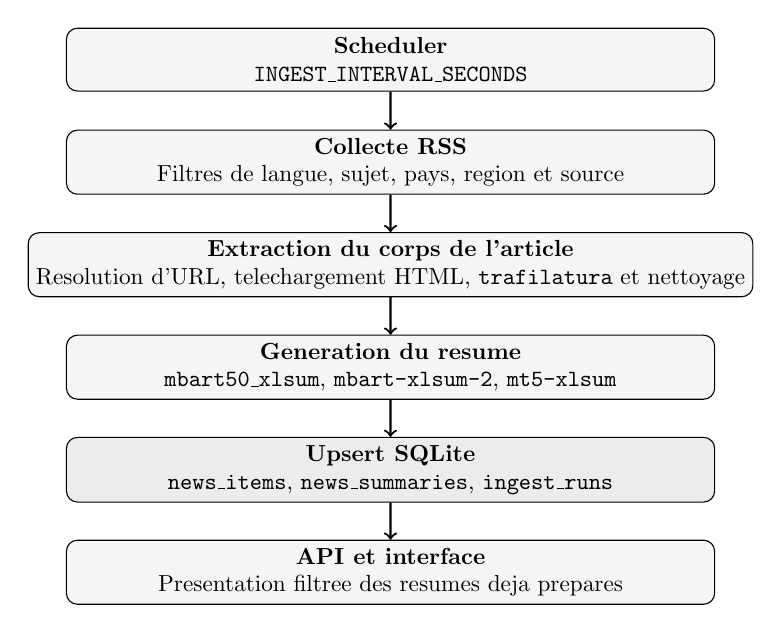
\begin{tikzpicture}[
  scale=0.84,
  every node/.style={transform shape},
  box/.style={draw, rounded corners, align=center, minimum width=9.8cm, minimum height=0.95cm, fill=gray!8},
  store/.style={draw, rounded corners, align=center, minimum width=9.8cm, minimum height=0.95cm, fill=gray!15},
  arrow/.style={->, thick}
]
\node[box] (scheduler) at (0,0) {
  \textbf{Scheduler}\\
  \texttt{INGEST\_INTERVAL\_SECONDS}
};
\node[box] (rss) at (0,-1.55) {
  \textbf{Collecte RSS}\\
  Filtres de langue, sujet, pays, region et source
};
\node[box] (article) at (0,-3.10) {
  \textbf{Extraction du corps de l'article}\\
  Resolution d'URL, telechargement HTML, \texttt{trafilatura} et nettoyage
};
\node[box] (summary) at (0,-4.65) {
  \textbf{Generation du resume}\\
  \texttt{mbart50\_xlsum}, \texttt{mbart-xlsum-2}, \texttt{mt5-xlsum}
};
\node[store] (db) at (0,-6.20) {
  \textbf{Upsert SQLite}\\
  \texttt{news\_items}, \texttt{news\_summaries}, \texttt{ingest\_runs}
};
\node[box] (api) at (0,-7.75) {
  \textbf{API et interface}\\
  Presentation filtree des resumes deja prepares
};
\draw[arrow] (scheduler) -- (rss);
\draw[arrow] (rss) -- (article);
\draw[arrow] (article) -- (summary);
\draw[arrow] (summary) -- (db);
\draw[arrow] (db) -- (api);
\end{tikzpicture}
\caption{Flux de collecte et de generation de resumes en arriere-plan}
\label{fig:ingest-flow-fr}
\end{figure}

\subsection{Couches de services}

L'application est organisee sous forme de couches de services. \texttt{NewsService} collecte les nouvelles RSS selon la langue et les filtres choisis. \texttt{ArticleService} tente d'extraire le texte principal et l'image a partir du lien de l'article. \texttt{SummarizationService} resume le texte nettoye avec le modele choisi et applique le post-traitement. \texttt{StorageService} stocke les articles, les resumes et les executions d'ingestion dans la base SQLite. \texttt{FeedService} recupere depuis la base les nouvelles a afficher dans l'interface et appelle le service de traduction si necessaire. \texttt{TranslationService} traduit le titre et le resume vers la langue cible.

La base de donnees contient trois tables principales. La table \texttt{news\_items} stocke le lien de l'article, la source, la langue, le sujet, le pays, la region, le titre, la date de publication, le lien de l'image et le texte de l'article. La table \texttt{news\_summaries} contient les resumes produits par modele pour chaque article. La table \texttt{ingest\_runs} enregistre la configuration, l'etat et les statistiques des executions d'ingestion en arriere-plan. L'unicite du lien d'article permet d'eviter l'insertion repetee du meme article.

\subsection{API et interface utilisateur}

Le principal endpoint de l'application est \texttt{GET /api/news}. Il accepte des parametres comme la langue, la langue de sortie, le sujet, le pays, la region, la source, le modele, le mot-cle et la limite de resultats. Pour les langues autres que l'anglais, seuls les modeles multilingues sont acceptes. En plus, \texttt{GET /api/ingest/status} retourne l'etat du scheduler et de la derniere execution d'ingestion, tandis que \texttt{POST /api/ingest/run} place immediatement une execution d'ingestion dans la file.

L'interface utilisateur propose des options pour choisir la langue, le type d'actualite, la region, le pays, la source, le mot-cle, le modele, la langue de sortie et l'affichage des images. Elle affiche le titre de l'article, le resume, le nom de la source, la date de publication, l'image et le lien vers la source originale. La conservation du lien original montre que le resume n'est pas presente comme une source definitive remplacant l'article, mais comme une aide a la lecture rapide.

\section{Qualite des sources et gestion des erreurs}

Les sources d'actualites reelles ne sont pas aussi regulieres que les jeux de donnees academiques. Certaines sources RSS peuvent etre inaccessibles, certaines pages d'articles peuvent ne pas fournir le texte complet, et certaines pages peuvent contenir de la publicite, de la navigation ou des repetitions de titre. Pour cette raison, plusieurs mesures de qualite et de gestion des erreurs ont ete mises en place.

Premierement, lorsque le texte complet ne peut pas etre extrait du lien de l'article, le systeme evite de resumer une entree vide ou de faible qualite. Deuxiemement, l'etape de nettoyage reduit les repetitions de titre, les phrases de metadata et les bruits propres aux sources. Troisiemement, si la generation produit un resume degenere ou presque identique au titre, le systeme rejette cette sortie et peut utiliser un resume extractif de secours. Quatriemement, un script de validation du pool de sources a ete prepare afin d'evaluer l'acces RSS, la longueur du corps de l'article, la qualite du texte et la capacite de resume.

\section{Limites de la methode}

Cette methode possede certaines limites. Premierement, le systeme n'est pas un systeme de fact-checking independant capable de verifier la verite externe d'une nouvelle. Les metriques de fidelite a la source et le score \texttt{quality\_factuality} sont des mesures proxy qui evaluent si le resume reste proche du texte source; elles ne garantissent pas la veracite de l'information dans le monde reel. Deuxiemement, les sources RSS sont souvent limitees aux nouvelles recentes; la couverture historique du systeme depend donc de l'historique fourni par chaque flux. Troisiemement, la performance des modeles multilingues varie selon la langue; un seul score general ne suffit donc pas pour prendre une decision valable pour toutes les langues.

Malgre ces limites, la methode correspond a l'objectif principal du projet: entrainer des modeles de resume d'actualites multilingues, les evaluer avec un modele de comparaison pret a l'emploi, analyser la qualite des resumes avec des metriques multidimensionnelles et integrer les modeles dans une application web fonctionnelle fournissant un flux d'actualites reel.
